\section{Developed Method}
\label{sec:HomographyDevelopedMethod}

The goal of our work was to offer a systematic way to select the ``best'' homography according to the proposed score function without any other prior knowledge about the quality of individual markers.

The method works like this. Each homography is induced by one independent marker. The input to our method is multiple sets (groups) of point correspondences between the warped and the ground-truth markers. So each set represents a marker. Our method can rank multiple homographies and select the best performing one according to the tailor-made score function. Thus, we require a homography matrix for each marker (a set of point correspondences). To compute these matrices, any state-of-the-art method can be utilized. The advantage of our method is that it can rank the referred homographies without the knowledge of absolute or relative positions of markers in the world. We did not propose any method to simultaneously estimate multiple homographies. We build upon the existing homography matrices.

Since we assume no knowledge about the arrangement of markers in the scene, we cannot virtually create one compound marker consisting of all the keypoints. If we could, then we would employ RANSAC or any other sophisticated algorithm to select the best subset of keypoints to estimate the homography. Our approach would be useless. But we only have information about the relative position of marker’s keypoints, not markers themselves. The point correspondence is globally indeterminate. We can only establish a local point correspondence between a single marker and its ground-truth shape. To obtain the isolated homographies, we suggest the user chooses the best method available.

The homography estimation between existing point correspondences is a standard problem and we heavily rely on its solutions. But we did not contribute to it in terms of improving the homography estimation itself. We provided a way to rank the resulting homographies according to our score function. We developed a way to,
under certain circumstances, choose the ``best'' homography from multiple existing ones. Therefore, our method could not even be compared to RANSAC, because we tackle a different problem.

The proposed method is based on the following assumptions:
\begin{enumerate}
    \item The markers are geometrically similar, i.e., they differ only in translation, rotation, and uniform scale in the real world.
    \item The shape of at least one of them is known.
    \item These markers are placed on the same planar surface in the scene.
\end{enumerate}
Our approach shows a way to relate all the markers to each other in a single score function without knowing their relative positions in the scene. Our method only handles transformation from a distorted to the undistorted view of the target plane. Thus, it serves for the removal of perspective distortion only.

We exploited the properties of homography and similarity transformations and expressed them in a single score function. This function stands at the core of our contribution. Its value is used as a proxy to rank homographies according to their reprojection error over the entire image using only markers' keypoints. The usual use case would be to select the homography with the lowest score, i.e., the highest-ranked matrix, to perform the image rectification.

\begin{figure}[t]
    \centerline{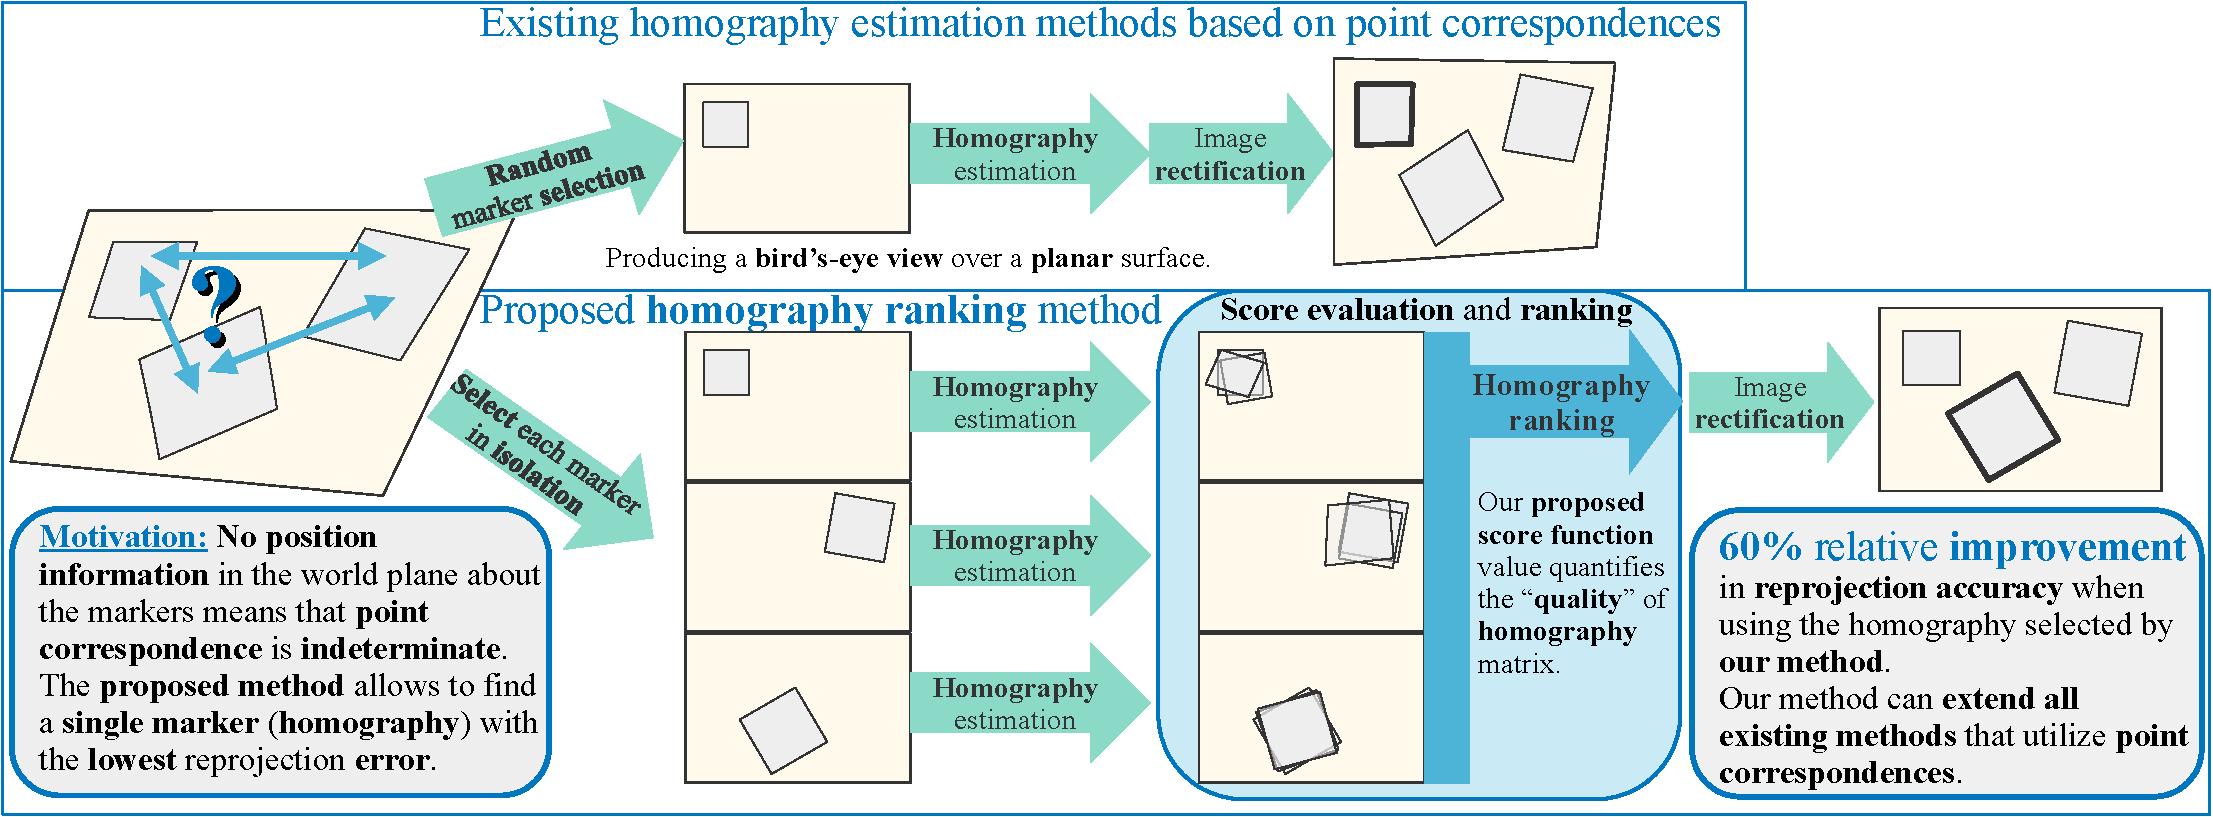
\includegraphics[width=\linewidth]{figures/homography/graphical_abstract.pdf}}
    \caption[Homography ranking graphical abstract]{Here we present the graphical abstract from our paper. The basic idea is that existing approaches may only estimate an isolated homography for each marker and cannot determine which homography achieves the best reprojection over the entire image. Therefore, we proposed a method to rank isolated homographies obtained from multiple distinct markers to select the best homography. This method extends existing approaches in the post-processing stage, provided that the point correspondences are available and the markers differ only by similarity transformation after rectification. We demonstrated the robustness of our method using a synthetic dataset and showed an approximately $60\%$ relative improvement over the random selection strategy based on the homography estimation from the OpenCV library.}
    \label{fig:GraphicalAbstract}
\end{figure}

\begin{figure}[t]
    \centerline{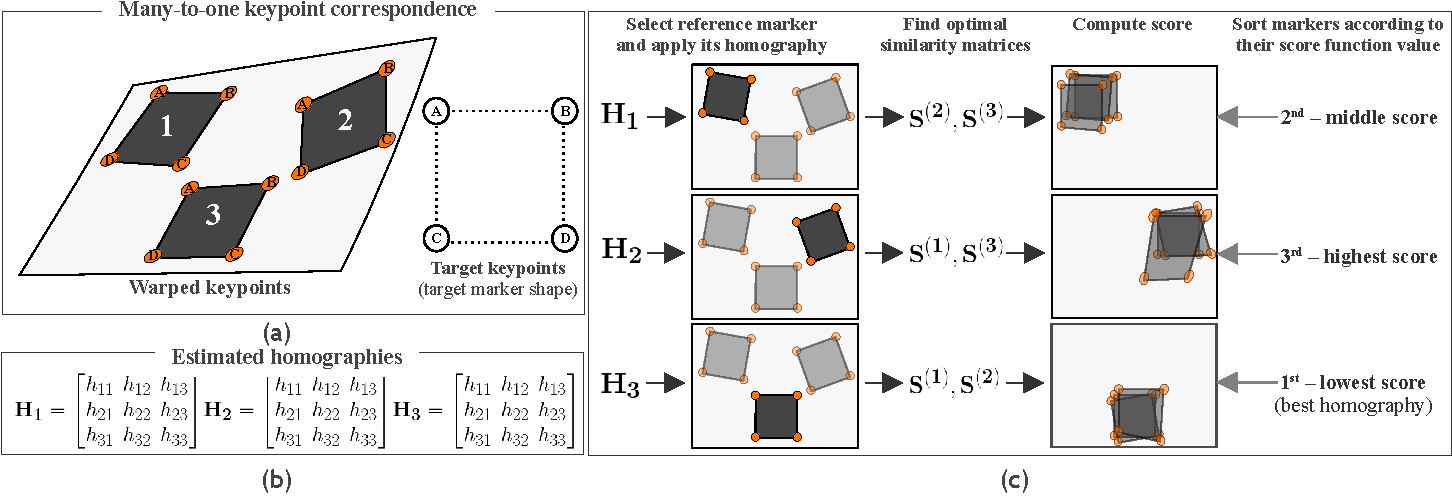
\includegraphics[width=\linewidth]{figures/homography/system_diagram.pdf}}
    \caption[Homography ranking system diagram]{A system diagram describing the general idea behind our method. \imgpartdesc{a} The input consists of a many-to-one point correspondence specified by geometrically similar markers and information about the shape of the target marker. \imgpartdesc{b} We assume that the isolated homographies corresponding to each independent marker are provided on the input as well. \imgpartdesc{c} The algorithm processes each marker by applying its homography matrix to the image to produce a rectified image. Subsequently, it computes optimal similarity matrices corresponding to the auxiliary markers. The computation of the score function makes use of these transformations. The obtained score values then serve for comparison to rank (sort in ascending order) the homographies. The homography ranked first is considered the ``best'' candidate for the minimal reprojection error over the entire image.}
    \label{fig:HomographySystemDiagram}
\end{figure}

Our algorithm is invariant to the underlying homography estimation method. It can thus serve as an extension to approaches that handle point correspondences, either as part of run time or a post-processing stage. Moreover, it is computationally very efficient, as it scales well with a quadratic complexity $\func{\Theta}{m^2}$.

Our method utilizes multiple similar markers (see Figure~\ref{fig:HomographySystemDiagram}). The input is point correspondences and homographies estimated for each marker. Each marker is selected exactly once as a \mbox{reference marker}. All remaining markers are in the role of \mbox{auxiliary markers}. The reference marker's homography is used to perform the perspective transformation to rectify all markers. To rank which reference markers' homography yields the best reprojection, we exploit auxiliary markers. Auxiliary markers are subsequently mapped onto the target marker using similarity transformations (equation~\eqref{eq:SimilarityMatrices}). We then convert the transformed keypoints to homogeneous coordinates and measure the reprojection error as the mean Euclidean distance between the rectified and the target keypoints~\eqref{eq:HomographyScoreFunction}. The aim is to minimize this quantity. The optimal similarity matrices are just auxiliary and redundant after the algorithm ends.

Let $r$ be the index of the reference marker. The $3 \times 3$ matrices describing similarity transformations are contained in a set $\mset{S} = \cbrackets{\suprbrackets{\mtx{S}}{i} \ |\ i = 1, \dots, m}$, such that

\begin{equation}
    \label{eq:SimilarityMatrices}
    \suprbrackets{\mtx{S}}{i} =
    \begin{cases}
        \begin{aligned}
             & \begin{bmatrix}
                1 & 0 & 0 \\
                0 & 1 & 0 \\
                0 & 0 & 1
            \end{bmatrix} & \text{if } i = r   \\
             & \begin{bmatrix}
                \subsuprbrackets{\mtx{R}}{2 \times 2}{i} & \subsuprbrackets{\mtx{T}}{2 \times 1}{i} \\
                \mathbf{0}_{1 \times 2}                  & 1
            \end{bmatrix} & \text{if }i \neq r \\
        \end{aligned}
    \end{cases},
\end{equation}

\noindent for $i = 1, \dots, m$, where

\begin{equation}
    \subsuprbrackets{\mtx{R}}{2 \times 2}{i} =
    \begin{bmatrix}
        \suprbrackets{s}{i} \cdot \func{\cos}{\suprbrackets{\theta}{i}} & -\suprbrackets{s}{i} \cdot \func{\sin}{\suprbrackets{\theta}{i}} \\
        \suprbrackets{s}{i} \cdot \func{\sin}{\suprbrackets{\theta}{i}} & \suprbrackets{s}{i} \cdot \func{\cos}{\suprbrackets{\theta}{i}}
    \end{bmatrix}, \quad
    \subsuprbrackets{\mtx{T}}{2 \times 1}{i} =
    \begin{bmatrix}
        \subsuprbrackets{t}{x}{i} \\
        \subsuprbrackets{t}{y}{i}
    \end{bmatrix}.
\end{equation}

\noindent This transformation (except for the identity) consists of $4$ DoF: single rotation angle $\suprbrackets{\theta}{i}$, two $x$ and $y$ translation coefficients $\subsuprbrackets{t}{x}{i}$, $\subsuprbrackets{t}{y}{i}$, and a scale coefficient $\suprbrackets{s}{i}$. A full affine transformation with $6$ DoF would be responsible for horizontal and vertical
scales, shear and rotation, and $x$, $y$ offsets~\cite{barath2016novel}. The application of homography that rectifies an image produces a frontal plane which is related to the ground-truth plane by similarity transformation~\cite{hartley2003multiple, beck2016planar}. Thus, we do not include the shear and we only support uniform scaling.

Since all the markers share the same planar surface, any homography has to provide a valid perspective projection, but all perspective projections are subjected to different noise. Our goal is to quantify which homography estimation provides the best perspective projection for the whole plane in the image. To do so, we propose a score function based on the aforementioned constraints. The score function computes a score for individual homographies in conjunction with estimated similarity matrices corresponding to auxiliary markers as

\begin{equation}
    \label{eq:HomographyScoreFunction}
    \func{\scoref}{\H, \mset{S}} =
    \frac{1}{m}
    \sum_{i = 1}^{m}
    \frobnorm{
        \func{h}{
            \suprbrackets{\mtx{S}}{i}
            \H
            \suprbrackets{\mtx{W}}{i}
        }
        -
        \mtx{T}
    },
\end{equation}

\noindent where $\frobnorm{\cdot}$ denotes the Frobenius norm. The function $\func{h}{\cdot}$ converts points to homogeneous coordinates as

\begin{equation}
    \label{eq:HomoCoordsConversion}
    \func{h}{
        \begin{bmatrix}
            x_1 & x_2 & \dots & x_k \\
            y_1 & y_2 & \dots & y_k \\
            z_1 & z_2 & \dots & z_k
        \end{bmatrix}
    } =
    \begin{bmatrix}
        \nicefrac{x_1}{z_1} & \nicefrac{x_2}{z_2} & \dots & \nicefrac{x_k}{z_k} \\
        \nicefrac{y_1}{z_1} & \nicefrac{y_2}{z_2} & \dots & \nicefrac{y_k}{z_k} \\
        1                   & 1                   & \dots & 1
    \end{bmatrix}.
\end{equation}

Now we describe the proposed Algorithm~\ref{alg:HomographyRanking} for homography ranking. Assume a set of warped markers described by warped keypoints and a single target marker described by target keypoints. These objects are linked by a many-to-one point correspondence. Also, assume that homographies have been estimated for each marker in isolation. Our algorithm ascendingly ranks the input set of all pairs $\rbrackets{\suprbrackets{\mtx{W}}{i}, \mtx{T}}$, $i = 1, \dots, m$, by how well each $i$-th marker preserves the target shape of all the markers in the image after removing the perspective distortion. This objective is measured by the score function defined in equation~\eqref{eq:HomographyScoreFunction}. The algorithm evaluates all markers as candidates for the reference marker. In each iteration, it computes optimal similarity matrices for the auxiliary markers in the rectified plane, i.e., after applying the perspective projection induced by the current homography. The aim is to find a homography with a minimal score. The algorithmic complexity is quadratic in the number of markers, thus $\func{\Theta}{m \rbrackets{m - 1} + m \func{\text{log}_2}{m}} \simeq \func{\Theta}{m^2}$.

\def\hmatrices{\boldsymbol{\bar{H}}}
\def\scoref{\mathcal{F}}

\begin{algorithm}[t]
    \caption{Homography Ranking}
    \label{alg:HomographyRanking}
    \begin{algorithmic}[1]
        \State $\hmatrices \gets \arraydef \left[ m \right]$
        \Comment{output array of homographies}

        \State $\scores \gets \arraydef \left[ m \right]$
        \Comment{array of scores}

        \For{$i \gets 1, \dots , m$}

        \State $\hmatrices \left[ i \right] \gets$
        \Call{homography}{$\suprbrackets{\mtx{W}}{i}$, $\mtx{T}$}
        \Comment{retrieve or estimate perspective}

        \State $\suprbrackets{\mtx{\bar{S}}}{i} \gets \mtx{I}_{3 \times 3}$

        \State $\mset{\bar{S}} \gets \cbrackets{\suprbrackets{\mtx{\bar{S}}}{i}}$
        \Comment{set of similarity matrices}

        \ForAll{$j$ : $\cbrackets{1, \dots, m} - \cbrackets{i}$}

        \State $\suprbrackets{\mtx{\bar{S}}}{j} \gets$ \Call{similarity}{$\hmatrices \left[ i \right] \cdot \suprbrackets{\mtx{W}}{j}$, $\mtx{T }$}

        \State$\mset{\bar{S}} \gets \mset{\bar{S}} \cup \suprbrackets{\mtx{\bar{S}}}{j}$
        \EndFor

        \State $\scores \left[ i \right] \gets \func{\scoref}{\hmatrices \left[ i \right], \mset{\bar{S}}}$
        \Comment{evaluate score function \eqref{eq:HomographyScoreFunction}}
        \EndFor
        \State $\sortres \gets \Call{argsort}{\scores}$
        \Comment{indirect sort}

        \State \Return $\hmatrices, \sortres$
    \end{algorithmic}
\end{algorithm}

It is important to note that the two functions used in this pseudocode to compute the homography and similarity matrices stand for arbitrary methods that produce the required transformations.

Our score function \eqref{eq:HomographyScoreFunction} is just a proxy for the reprojection error computed over the whole image. Since we utilize only a small subset of points from the entire image, which may be subjected to noise, the assumption that the ``best'' homography is the one our method ranks as first may not hold in every case. In very few cases, the marker that achieves the lowest score function value does indeed reconstruct the remaining markers the best, but not the overall image. However, our experiments show that our method consistently preserves its performance under various conditions.
